% !TEX root = SystemTemplate.tex

\chapter{Overview and concept of operations}

This report covers the project overview, user stories, backlog, design and implementation, development environment, deployment, and documentation for the testing project. 


\section{Scope}
This section gives a brief overview of the system.


\section{Purpose}
The purpose of this program is to run {\tt .cpp} files with given test files, and grade them. 


\subsection{Traversing Subdirectories}
Traversing subdirectories is one of the main components of this system. The program runs a {\tt .cpp} file using test files, and the test files are stored in the current and all the subdirectories.  

\subsection{Running the Program Using Test Cases}
The software was designed in the Linux environment provided to the group by the university. 
 

\section{Systems Goals}
The goal of this system is to grade a {\tt .cpp} file just by typing {\tt grade <filename>.cpp}. The product is built to test the {\tt .cpp} file with all the given {\tt .tst} test files in the current directory and all the subdirectories, and compare the results to the corresponding {\tt .ans} files.  

\section{System Overview and Diagram}
Here is a flow diagram showing the implementation process:

\begin{figure}[tbh]
\begin{center}
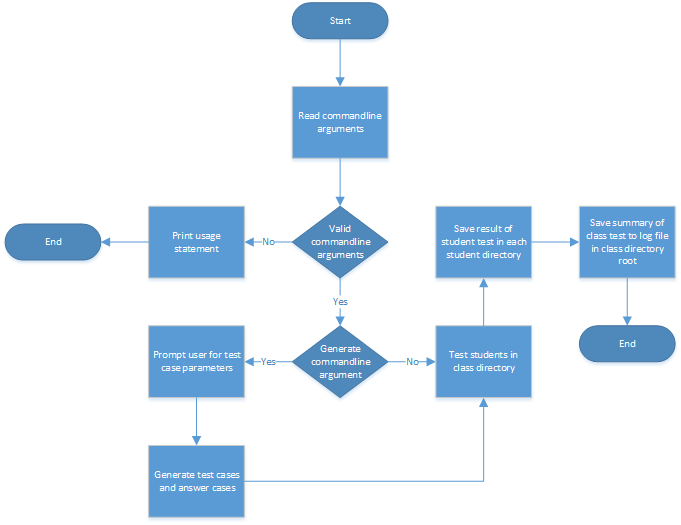
\includegraphics[width=1\textwidth]{./SystemDiagram}
\end{center}
\caption{System Diagram \label{systemdiagram}}
\end{figure}




